\documentclass[a4paper]{article}
\usepackage{fullpage}
\usepackage[dvipsnames]{xcolor}
\usepackage{url}
\usepackage{tikz}
\usepackage{tikzpeople}
  \usepackage[
    backend=biber,
    style=numeric,
  ]{biblatex}

 \addbibresource{thispaper.bib}
% The basic structure of the figure as drawn in \basic is an extension of the structure in Tikzpeople of Nils Fleischhacker and some figure from openclipart. See the references for the link to the tikzpeople package. I could not access the openclipart website due to bad certificate. 
\newcommand{\human}[2]{
\definecolor{myskin}{named}{#1};

	\tikzset{		myskin/.style=        {color=myskin,top color=myskin!70, bottom color=myskin,shading angle=45}}
	
% \node[mexican,minimum size=2.5cm] (M) at (0pt,-250pt) {A
% Mexican};
\draw[myskin]
  (-60.0pt,-60.0pt) .. controls (-56pt,-64pt) and (-53pt,-68pt)..
  (-40pt,-68pt) .. controls (-40pt,-80pt)  and (-40pt,-90pt)..
  (-30pt,-110pt) .. controls (0pt,-120pt) and (30pt,-110pt) ..
  ( 30pt,-110pt) .. controls (40pt,-90pt)  and (40pt,-80pt)..
  (40pt,-68pt) .. controls (53pt,-68pt) and (56pt,-64pt)..
  ( 60pt,-60pt) .. controls ( 50pt, 0pt) and (-50pt, 0pt) .. 
		(-60pt,-60pt) -- cycle;
 %%%%%%%%%%%% The following lacks proportion%%%%%%%%%%%
  % \draw[myskin]
  % (-60.0pt,-60.0pt) .. controls (-56pt,-64pt) and (-53pt,-68pt)..
  % (-40pt,-68pt) .. controls (-40pt,-80pt)  and (-40pt,-90pt)..
  % (-30pt,-100pt) .. controls (0pt,-110pt) and (30pt,-100pt) ..
  % ( 30pt,-100pt) .. controls (40pt,-90pt)  and (40pt,-80pt)..
  % (40pt,-68pt) .. controls (53pt,-68pt) and (56pt,-64pt)..
  % ( 60pt,-60pt) .. controls ( 50pt, 0pt) and (-50pt, 0pt) .. 
		% (-60pt,-60pt) -- cycle;
  %%%%%%%%%%%%%%%%%%%%%%%%%%%%%%%%%%%%%%%%%%%%%%%%%%%%%%%%

  \draw[myskin] (0pt,0pt) ellipse (30pt and 27pt);
% \draw[fill=white](0pt,-50pt) ellipse (18pt and 13pt);
% \clip (0pt,-50pt) ellipse (16pt and 12pt) node {
\includegraphics[width=.11\textwidth]{flags/in.png}};

\draw[fill=white](0pt,-65pt) circle (28pt);
\clip (0pt,-65pt) circle (24pt) node {\includegraphics[width=.04\textwidth]{#2}};
}


%%%%%%%%%%%%%%%% This is for nationals. the badges are scaled with a larger height
\newcommand{\national}[2]{
\definecolor{myskin}{named}{#1};

	\tikzset{		myskin/.style=        {color=myskin,top color=myskin!70, bottom color=myskin,shading angle=45}}
	
% \node[mexican,minimum size=2.5cm] (M) at (0pt,-250pt) {A
% Mexican};
\draw[myskin]
  (-60.0pt,-60.0pt) .. controls (-56pt,-64pt) and (-53pt,-68pt)..
  (-40pt,-68pt) .. controls (-40pt,-80pt)  and (-40pt,-90pt)..
  (-30pt,-110pt) .. controls (0pt,-120pt) and (30pt,-110pt) ..
  ( 30pt,-110pt) .. controls (40pt,-90pt)  and (40pt,-80pt)..
  (40pt,-68pt) .. controls (53pt,-68pt) and (56pt,-64pt)..
  ( 60pt,-60pt) .. controls ( 50pt, 0pt) and (-50pt, 0pt) .. 
		(-60pt,-60pt) -- cycle;
 %%%%%%%%%%%% The following lacks proportion%%%%%%%%%%%
  % \draw[myskin]
  % (-60.0pt,-60.0pt) .. controls (-56pt,-64pt) and (-53pt,-68pt)..
  % (-40pt,-68pt) .. controls (-40pt,-80pt)  and (-40pt,-90pt)..
  % (-30pt,-100pt) .. controls (0pt,-110pt) and (30pt,-100pt) ..
  % ( 30pt,-100pt) .. controls (40pt,-90pt)  and (40pt,-80pt)..
  % (40pt,-68pt) .. controls (53pt,-68pt) and (56pt,-64pt)..
  % ( 60pt,-60pt) .. controls ( 50pt, 0pt) and (-50pt, 0pt) .. 
		% (-60pt,-60pt) -- cycle;
  %%%%%%%%%%%%%%%%%%%%%%%%%%%%%%%%%%%%%%%%%%%%%%%%%%%%%%%%

  \draw[myskin] (0pt,0pt) ellipse (30pt and 27pt);
% \draw[fill=white](0pt,-50pt) ellipse (18pt and 13pt);
% \clip (0pt,-50pt) ellipse (16pt and 12pt) node {
\includegraphics[width=.11\textwidth]{flags/in.png}};

\draw[fill=white](0pt,-60pt) circle (24pt);
\clip (0pt,-60pt) circle (22pt) node {\includegraphics[width=.07\textwidth]{#2}};
}

%%%%%%%%%%%%%%%% This is for basic. no badge
\newcommand{\basic}[1]{
\definecolor{myskin}{named}{#1};

	\tikzset{		myskin/.style=        {color=myskin,top color=myskin!70, bottom color=myskin,shading angle=45}}
	
% \node[mexican,minimum size=2.5cm] (M) at (0pt,-250pt) {A
% Mexican};
\draw[myskin]
  (-60.0pt,-60.0pt) .. controls (-56pt,-64pt) and (-53pt,-68pt)..
  (-40pt,-68pt) .. controls (-40pt,-80pt)  and (-40pt,-90pt)..
  (-30pt,-110pt) .. controls (0pt,-120pt) and (30pt,-110pt) ..
  ( 30pt,-110pt) .. controls (40pt,-90pt)  and (40pt,-80pt)..
  (40pt,-68pt) .. controls (53pt,-68pt) and (56pt,-64pt)..
  ( 60pt,-60pt) .. controls ( 50pt, 0pt) and (-50pt, 0pt) .. 
		(-60pt,-60pt) -- cycle;
 %%%%%%%%%%%% The following lacks proportion%%%%%%%%%%%
  % \draw[myskin]
  % (-60.0pt,-60.0pt) .. controls (-56pt,-64pt) and (-53pt,-68pt)..
  % (-40pt,-68pt) .. controls (-40pt,-80pt)  and (-40pt,-90pt)..
  % (-30pt,-100pt) .. controls (0pt,-110pt) and (30pt,-100pt) ..
  % ( 30pt,-100pt) .. controls (40pt,-90pt)  and (40pt,-80pt)..
  % (40pt,-68pt) .. controls (53pt,-68pt) and (56pt,-64pt)..
  % ( 60pt,-60pt) .. controls ( 50pt, 0pt) and (-50pt, 0pt) .. 
		% (-60pt,-60pt) -- cycle;
  %%%%%%%%%%%%%%%%%%%%%%%%%%%%%%%%%%%%%%%%%%%%%%%%%%%%%%%%

  \draw[myskin] (0pt,0pt) ellipse (30pt and 27pt);
% \draw[fill=white](0pt,-50pt) ellipse (18pt and 13pt);
% \clip (0pt,-50pt) ellipse (16pt and 12pt) node {
\includegraphics[width=.11\textwidth]{flags/in.png}};
}


\definecolor{nhs-green}{RGB}{0,103,71}
\definecolor{nhs-blue}{RGB}{0,94,184}
\definecolor{jeans}{RGB}{21,96,179}
\title{(De)-humanizing Clip arts}
\author{Rishiraj Bhattacharyya}
\date{October 1, 2023}
\begin{document}
\maketitle
\thispagestyle{empty}
\newpage
\section{Motivation}
Modern presentations live on clip arts. Since mid-90s quite a lot of human effort has gone into making clip arts more lively, aiming towards perhaps more realistic slide-designs. TikzPeople~\cite{TikzPeople}, a latex package written in TikZ by a cryptographer colleague, includes amazing designs for shapes of people to depict different characters in slides. The design principle follows the immensely popular type of clip arts included in the Microsoft Visio software. TikzPeople got so popular that it now comes bundled with TexLive.

While preparing for my presentations (in conferences and classroom lectures), I wanted to design EDI-aware slides. While exploring different options in TikzPeople, I noticed the following comments in the documentation (under the option female)~\cite{Manual} 
\begin{verbatim}
   The female option is supposed to make stereotypically male nodes look just tad more 
   feminine. For most tikzpeople this is accomplished by adding longer hair and losing
   the beard - though surprisingly, evil women still tend to have a goatee.

   This is useful to avoid being called sexist for not having women in you figures. On 
   the other hand people can now accuse you of enforcing gender stereotypes. 
   So have fun.
\end{verbatim}
These comments, at the very least, prove the limitations of the design principles used in TikzPeople and perhaps broadly, the design philosophy of the clip arts in the Microsoft Visio software. Indeed the characters are depicted via the \emph{skin colour}, \emph{physical features like hair and beard length and colour} and \emph{professional uniform/national dress}. The mexican node in TikzPeople is a very good example. 

\begin{figure}[h]
    \centering
    
\begin{tikzpicture}
        \node[mexican, minimum size=1.5cm] {};
    \end{tikzpicture}
    \label{fig:tikzpeople-mexican}
    \caption{ A mexican in TikzPeople}
\end{figure}
Such a stereotypical description of any national in any lecture slide is surely improper. I needed to design my own clip arts.


\section{Tikzclip}
In this Tikzclip project, I attempt to create a set of TikZ clip arts which would support diversity and inclusivity. The design principle is simple: the figures would be \emph{abstract} and the individual characters are depicted by the \emph{tools} of the trade or the \emph{flags} of the country. 

The basic design is the following abstract figure. As we do not aim to accurately draw any specific body part, we could use any colour available to us via the xcolor package.

\begin{figure}[htb]
    \centering
    
\begin{tikzpicture}
        \begin{scope}[scale=0.5]
            \basic{Tan}
        \end{scope}
        \begin{scope}[scale=0.5, xshift=5cm]
            \basic{CornflowerBlue}
        \end{scope}
        \begin{scope}[scale=0.5, xshift=10cm]
            \basic{OliveGreen}
        \end{scope}
    \end{tikzpicture}
     \caption{ Our Design: The Basic Figures in Different Colors}
    \label{fig:Tikzclip-basic}
   \end{figure}

To represent any national, the idea is to fix a badge with the corresponding national flag. Thus a mexican, using Tikzclip could be depicted as in Figure~\ref{fig:Tikzclip-mexican}.

\begin{figure}[htb]
    \centering
    \begin{tikzpicture}
        \begin{scope}[scale=0.5]
            \national{Tan}{flags/mx.png}
        \end{scope}
         \begin{scope}[scale=0.5,xshift=5cm]
            \national{CornflowerBlue}{flags/mx.png}
        \end{scope}
         \begin{scope}[scale=0.5, xshift=10cm]
            \national{OliveGreen}{flags/mx.png}
        \end{scope}
        
    \end{tikzpicture}
       \caption{ Our Design: Mexicans in Tikzclip}
    \label{fig:Tikzclip-mexican}
 
\end{figure}

To represent any professional, the badge could be the tools they use. For example, a microscope could be a good badge to depict a scientist, a cycle could be used to depict a cyclist, and musical notations are candidate symbol for singers. 

\begin{figure}[htb]
    \centering
    \begin{tikzpicture}
        \begin{scope}[scale=0.5]
            \human{Tan}{microscope.png}
        \end{scope}
         \begin{scope}[scale=0.5,xshift=5cm]
            \human{CornflowerBlue}{bike0.png}
        \end{scope}
         \begin{scope}[scale=0.5, xshift=10cm]
            \human{OliveGreen}{music2.png}
        \end{scope}
        
    \end{tikzpicture}
    \label{fig:Tikzclip-profession}
    \caption{ A scientist, a Cyclist, and a Singer}
\end{figure}

Of course, we may pick out some different tool for the badge, by using a different picture.

\begin{figure}[htb]
    \centering
    \begin{tikzpicture}
        \begin{scope}[scale=0.5]
            \human{Fuchsia}{chem5.jpeg}
        \end{scope}
         \begin{scope}[scale=0.5,xshift=5cm]
            \human{YellowOrange}{cycle1.png}
        \end{scope}
         \begin{scope}[scale=0.5, xshift=10cm]
            \human{Maroon}{mic4.png}
        \end{scope}
        
    \end{tikzpicture}
    \label{fig:Tikzclip-profession2}
    \caption{ A scientist, a Cyclist, and a Singer}
\end{figure}
\section{Source Code}
Source code of the Tikzclip project is available at \url{https://github.com/rishirajb/tikzclip}. Please feel free to modify and use.  
  \printbibliography
\newpage
\begin{tikzpicture}

\begin{scope}
\node(title1) at (0pt,300pt) {{\textbf{Character}}};
\node(title2) at (180pt,300pt) {{\textbf{Our Design}}};
\node(title2) at (380pt,300pt) {{\textbf{TikzPeople}}};
 \node (l1) at (0pt,-250pt) {\large{Doctor}};
  \node (l2) at (0pt,-125pt) {\large{Nurse}};
   \node (l3) at (0pt,0pt) {\large{Builder}};
 \node (l5) at (0pt,250pt) {\large{Pilot}};
  \node (l4) at (0pt,125pt) {\large{Chef}};
   
\end{scope}


\begin{scope}[xshift=200pt]
\node[physician,female,minimum size=1.5cm] (M1) at (180pt,-250pt) {};
\node[nurse,female,minimum size=1.5cm] (M2) at (180pt,-125pt) {};
\node[chef,minimum size=1.5cm] (M4) at (180pt,125pt) {};
\node[builder,minimum size=1.5cm] (M3) at (180pt,0pt) {};
\node[pilot, hair=gray, minimum
size=1.5cm] (M5) at (180pt,250pt) {};
\end{scope}

\begin{scope}[scale=0.5,xshift=400pt,yshift=-450pt]
    \human{nhs-blue}{doctor2.png}
\end{scope}

\begin{scope}[scale=0.5,xshift=400pt,yshift=-215pt]
    \human{nhs-green}{nurse.png}
\end{scope}

\begin{scope}[scale=0.5,xshift=400pt,yshift=40pt]
    \human{jeans}{labour.png}
\end{scope}
\begin{scope}[scale=0.5,xshift=400pt,yshift=295pt]
    \human{gray}{chefhat.png}
\end{scope}
\begin{scope}[scale=0.5,xshift=400pt,yshift=530pt]
    \human{RawSienna}{plane2.png}
\end{scope}

\end{tikzpicture}
\newpage 
\section{If you want to depict a British Person}
Choose any colour you want...

\vspace*{2cm}
\begin{tikzpicture}
\begin{scope}[scale=0.5]
\national{Tan}{flags/gb.png}
\end{scope}
\begin{scope}[scale=0.5,xshift=-130pt]
\national{Green}{flags/gb.png}
\end{scope}
\begin{scope}[scale=0.5,xshift=130pt]
\national{Blue}{flags/gb.png}
\end{scope}
\begin{scope}[scale=0.5,xshift=260pt]
\national{Black }{flags/gb.png}
\end{scope}

 \begin{scope}[scale=0.5,yshift=200pt]
\national{Mahogany}{flags/gb.png}
\end{scope}
\begin{scope}[scale=0.5,xshift=-130pt, yshift=200pt]
\national{OliveGreen}{flags/gb.png}
\end{scope}
\begin{scope}[scale=0.5,xshift=130pt,yshift=200pt]
\national{NavyBlue}{flags/gb.png}
\end{scope}
\begin{scope}[scale=0.5,xshift=260pt,yshift=200pt]
\national{Sepia}{flags/gb.png}
\end{scope}
\begin{scope}[scale=0.5,xshift=520pt, yshift=200pt]
\national{Mulberry}{flags/gb.png}
\end{scope}
\begin{scope}[scale=0.5, xshift=390pt, yshift=200pt]
\national{PineGreen}{flags/gb.png}
\end{scope}
\begin{scope}[scale=0.5, xshift=520pt]
\national{MidnightBlue}{flags/gb.png}
\end{scope}
\begin{scope}[scale=0.5, xshift=390pt]
\national{Bittersweet}{flags/gb.png}
\end{scope}
 
% \node[inner sep=0pt] (russell) at (0pt,-60pt) {
\includegraphics[width=.08\textwidth]{flags/mx.png}};
\end{tikzpicture}
\end{document}

\newpage
\begin{tikzpicture}[xshift=20cm]
\definecolor{myskin}{named}{Blue};

	\tikzset{ myskin/.style=        {color=myskin,top color=myskin!70, bottom color=myskin,shading angle=45}}
	
% \node[mexican,minimum size=2.5cm] (M) at (0pt,-250pt) {A
% Mexican};
\draw[myskin]
  (-60.0pt,-60.0pt) .. controls (-56pt,-64pt) and (-53pt,-68pt)..
  (-40pt,-68pt) .. controls (-40pt,-80pt)  and (-40pt,-90pt)..
  (-30pt,-110pt) .. controls (0pt,-120pt) and (30pt,-110pt) ..
  ( 30pt,-110pt) .. controls (40pt,-90pt)  and (40pt,-80pt)..
  (40pt,-68pt) .. controls (53pt,-68pt) and (56pt,-64pt)..
  ( 60pt,-60pt) .. controls ( 50pt, 0pt) and (-50pt, 0pt) .. 
		(-60pt,-60pt) -- cycle;
 %%%%%%%%%%%% The following lacks proportion%%%%%%%%%%%
  % \draw[myskin]
  % (-60.0pt,-60.0pt) .. controls (-56pt,-64pt) and (-53pt,-68pt)..
  % (-40pt,-68pt) .. controls (-40pt,-80pt)  and (-40pt,-90pt)..
  % (-30pt,-100pt) .. controls (0pt,-110pt) and (30pt,-100pt) ..
  % ( 30pt,-100pt) .. controls (40pt,-90pt)  and (40pt,-80pt)..
  % (40pt,-68pt) .. controls (53pt,-68pt) and (56pt,-64pt)..
  % ( 60pt,-60pt) .. controls ( 50pt, 0pt) and (-50pt, 0pt) .. 
		% (-60pt,-60pt) -- cycle;
  %%%%%%%%%%%%%%%%%%%%%%%%%%%%%%%%%%%%%%%%%%%%%%%%%%%%%%%%

  \draw[myskin] (0pt,0pt) ellipse (30pt and 27pt);
% \draw[fill=white](0pt,-50pt) ellipse (18pt and 13pt);
% \clip (0pt,-50pt) ellipse (16pt and 12pt) node {
\includegraphics[width=.11\textwidth]{flags/in.png}};

\draw[fill=white](0pt,-60pt) circle (20pt);
\clip (0pt,-60pt) circle (19pt) node {
\includegraphics[width=.12\textwidth]{flags/mx.png}};

 
% \node[inner sep=0pt] (russell) at (0pt,-60pt) {
\includegraphics[width=.08\textwidth]{flags/mx.png}};
\end{tikzpicture}
\newpage

\begin{tikzpicture}
\definecolor{myskin}{named}{blue};

	\tikzset{		myskin/.style=        {color=myskin,top color=myskin!70, bottom color=myskin,shading angle=45}}
	
\node[builder,minimum size=2.5cm] (M) at (0pt,-250pt) {A
Builder};
  \draw[myskin]
  (-60.0pt,-60.0pt) .. controls (-56pt,-64pt) and (-53pt,-68pt)..
  (-40pt,-68pt) .. controls (-40pt,-80pt)  and (-40pt,-90pt)..
  (-30pt,-110pt) .. controls (0pt,-120pt) and (30pt,-110pt) ..
  ( 30pt,-110pt) .. controls (40pt,-90pt)  and (40pt,-80pt)..
  (40pt,-68pt) .. controls (53pt,-68pt) and (56pt,-64pt)..
  ( 60pt,-60pt) .. controls ( 50pt, 0pt) and (-50pt, 0pt) .. 
		(-60pt,-60pt) -- cycle;
  \draw[myskin] (0pt,0pt) ellipse (30pt and 27pt);
% \draw[fill=white](0pt,-50pt) ellipse (18pt and 13pt);
% \clip (0pt,-50pt) ellipse (16pt and 12pt) node {
\includegraphics[width=.11\textwidth]{flags/in.png}};


\draw[fill=white](0pt,-60pt) circle (20pt);
\clip (0pt,-60pt) circle (19pt) node {
\includegraphics[width=.09\textwidth]{labour.png}};


 
%\node[inner sep=0pt] (russell) at (0pt,-55pt) {
\includegraphics[width=.08\textwidth]{labour.png}};
\end{tikzpicture}
\newpage

\begin{tikzpicture}
\definecolor{myskin}{named}{nhs-blue};
%MidnightBlue
	\tikzset{		myskin/.style=        {color=myskin,top color=myskin!70, bottom color=myskin,shading angle=45}}
	
\node[physician,female,minimum size=2.5cm] (M) at (0pt,-250pt) {A
Doctor};
  \draw[myskin]
  (-60.0pt,-60.0pt) .. controls (-56pt,-64pt) and (-53pt,-68pt)..
  (-40pt,-68pt) .. controls (-40pt,-80pt)  and (-40pt,-90pt)..
  (-30pt,-110pt) .. controls (0pt,-120pt) and (30pt,-110pt) ..
  ( 30pt,-110pt) .. controls (40pt,-90pt)  and (40pt,-80pt)..
  (40pt,-68pt) .. controls (53pt,-68pt) and (56pt,-64pt)..
  ( 60pt,-60pt) .. controls ( 50pt, 0pt) and (-50pt, 0pt) .. 
		(-60pt,-60pt) -- cycle;
  \draw[myskin] (0pt,0pt) ellipse (30pt and 27pt);
% \draw[fill=white](0pt,-50pt) ellipse (18pt and 13pt);
% \clip (0pt,-50pt) ellipse (16pt and 12pt) node {
\includegraphics[width=.11\textwidth]{flags/in.png}};


\draw[fill=white](0pt,-55pt) circle (18pt);
\clip (0pt,-55pt) circle (17pt) node {
\includegraphics[width=.07\textwidth]{doctor2.png}};


 
%\node[inner sep=0pt] (russell) at (0pt,-55pt) {
\includegraphics[width=.08\textwidth]{labour.png}};
\end{tikzpicture}


\newpage

\begin{tikzpicture}
\definecolor{myskin}{named}{nhs-green};


	\tikzset{		myskin/.style=        {color=myskin,top color=myskin!70, bottom color=myskin,shading angle=45}}
	
\node[nurse,female,minimum size=2.5cm] (M) at (0pt,-250pt) {A
Nurse};
  \draw[myskin]
  (-60.0pt,-60.0pt) .. controls (-56pt,-64pt) and (-53pt,-68pt)..
  (-40pt,-68pt) .. controls (-40pt,-80pt)  and (-40pt,-90pt)..
  (-30pt,-110pt) .. controls (0pt,-120pt) and (30pt,-110pt) ..
  ( 30pt,-110pt) .. controls (40pt,-90pt)  and (40pt,-80pt)..
  (40pt,-68pt) .. controls (53pt,-68pt) and (56pt,-64pt)..
  ( 60pt,-60pt) .. controls ( 50pt, 0pt) and (-50pt, 0pt) .. 
		(-60pt,-60pt) -- cycle;
  \draw[myskin] (0pt,0pt) ellipse (30pt and 27pt);
% \draw[fill=white](0pt,-50pt) ellipse (18pt and 13pt);
% \clip (0pt,-50pt) ellipse (16pt and 12pt) node {
\includegraphics[width=.11\textwidth]{flags/in.png}};


\draw[fill=white](0pt,-55pt) circle (18pt);
\clip (0pt,-55pt) circle (17pt) node {
\includegraphics[width=.07\textwidth]{nurse.png}};


 
%\node[inner sep=0pt] (russell) at (0pt,-55pt) {
\includegraphics[width=.08\textwidth]{labour.png}};
\end{tikzpicture}

\documentclass{article}
\usepackage{tikz}
\begin{document}
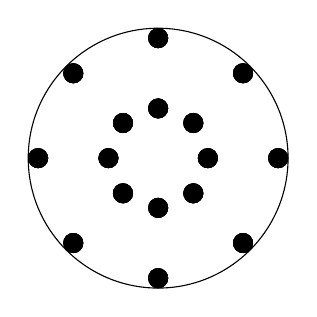
\begin{tikzpicture}
    \draw[fill=white] (0,0) circle (1.65);
    
    \foreach \x in {0,45,...,315}
        \foreach \y in {22.5,67.5,...,337.5}
            \draw[fill=black] ({1.65*cos(\x)*sin(\y)}, {1.65*sin(\x)*sin(\y)}) circle (0.12);
\end{tikzpicture}
\end{document}